\section{Linearization, critical points, and equilibria}
\label{linearization:section}

\LAtt{8.1}

\LO{
\item Find critical points of a non-linear system of differential equations and
\item Linearize a non-linear system around a critical point by computing the Jacobian matrix. 
}

%\subsection{Nonlinear equations}

Except for a few brief detours in \chapterref{fo:chapter},
we considered mostly linear
equations.  Linear equations suffice in many applications, but in reality
most phenomena require nonlinear equations.  Nonlinear equations, however,
are notoriously more difficult to understand than linear ones, and 
many strange new phenomena appear when we allow our equations to be
nonlinear.

Not to worry, we did not waste all this time studying linear equations.
Nonlinear equations can often be approximated by linear ones if we only need
a solution \myquote{locally,} for example, only for a short period of time, or
only for certain parameters.  Understanding specific linear equations can
also give us qualitative understanding about a more general nonlinear
problem.  The idea is similar to what you did in calculus in trying to
approximate a function by a line with the right slope.

\begin{mywrapfigsimp}{1.45in}{1.75in}
\noindent
\inputpdft{mv-pend}
\end{mywrapfigsimp}
In \sectionref{sec:mv} we looked at the pendulum of %mass $m$ and
length $L$.  The goal was to solve for the angle $\theta(t)$ as
a function of the time $t$.  The equation for the setup is
the nonlinear equation
\begin{equation*}
\theta'' + \frac{g}{L} \sin \theta = 0 .
\end{equation*}
Instead of solving this equation, we solved the rather easier linear
equation
\begin{equation*}
\theta'' + \frac{g}{L} \theta = 0 .
\end{equation*}
While the solution to the linear equation is not exactly what we were
looking for, it is rather close to the original, as long as the
angle $\theta$ is small and the time period involved is short.

You might ask: Why don't we just solve the nonlinear problem?  Well, it
might be very difficult, impractical, or impossible to solve analytically,
depending on the equation in question.  We may
not even be interested in the actual solution, we might only be interested
in some qualitative idea of what the solution is doing.  For example,
%we may be interested in
what happens as time goes to infinity?
%In the case
%of the pendulum we found that it oscillates and we can even approximate
%the period well if the swings are small.
%In other words, why do more work, when we can do less.
%The exact solution, even if found, might be harder to analyze.


\subsection{Autonomous systems and phase plane analysis}

We restrict our attention to a two-dimensional autonomous system
\begin{equation*}
x' = f(x,y) , \qquad y' = g(x,y) ,
\end{equation*}
where $f(x,y)$ and $g(x,y)$ are functions of two variables, and the
derivatives are taken with respect to time $t$.  Solutions are
functions $x(t)$ and $y(t)$ such that
\begin{equation*}
x'(t) = f\bigl(x(t),y(t)\bigr), \qquad
y'(t) = g\bigl(x(t),y(t)\bigr) .
\end{equation*}
The way we will analyze the system is very similar to
\sectionref{auteq:section}, where we studied a single autonomous equation.  The
ideas in two dimensions are the same, but the behavior can be
far more complicated.
%We will do the same sort of analysis.  We will
%look for the \emph{critical points} of the system and then we will analyze
%what happens when time goes to infinity.

It may be best to think of the system of equations as the single vector equation
\begin{equation} \label{eq:nlinautn2}
\begin{bmatrix} x \\ y \end{bmatrix} ' =
\begin{bmatrix} f(x,y) \\ g(x,y) \end{bmatrix} .
\end{equation}
As in \sectionref{sec:introtosys} we draw
the \emph{\myindex{phase portrait}} (or \emph{\myindex{phase diagram}}),
where each point $(x,y)$ corresponds to a specific state of the system.
We draw the \emph{\myindex{vector field}}
given at each
point $(x,y)$ by the vector
$\left[ \begin{smallmatrix} f(x,y) \\ g(x,y) \end{smallmatrix} \right]$.
And as before if we find solutions, we draw the trajectories
by plotting all points $\bigl(x(t),y(t)\bigr)$ for a certain range of $t$.

\begin{example} \label{example:nlin-1b-example}
Consider the second order equation $x''=-x+x^2$.
Write this equation as a first order nonlinear system
\begin{equation*}
x' = y , \qquad y' = -x+x^2 .
\end{equation*}
The phase portrait with some trajectories is drawn in
\figurevref{fig:nlin-1b}.
\begin{myfig}
\capstart
\diffyincludegraphics{width=3in}{width=4.5in}{nlin-1b}
\caption{Phase portrait with some trajectories of
$x' = y$, $y' = -x+x^2$. \label{fig:nlin-1b}}
\end{myfig}

From the phase portrait it should be clear that even this simple system has
fairly complicated behavior.  Some trajectories keep oscillating around the
origin, and some go off towards infinity.  We will return to this example
often, and analyze it completely in this (and the next) section.
\end{example}

If we zoom into the diagram near a point where 
$\left[ \begin{smallmatrix} f(x,y) \\ g(x,y) \end{smallmatrix} \right]$ is
not zero, then nearby the arrows point generally in essentially that same
direction and have essentially the same magnitude.
In other words the behavior is not that interesting near such a point.
We are of course assuming that $f(x,y)$ and $g(x,y)$ are continuous.

Let us concentrate on those points in the phase diagram
above where the trajectories
seem to start, end, or go around.  We see two such points:
$(0,0)$ and $(1,0)$.  The trajectories seem to go around the point $(0,0)$,
and they seem to either go in or out of the point $(1,0)$.
%
These points are precisely those points where the derivatives of both $x$
and $y$ are zero.  

\begin{definition} The \emph{critical points}\index{critical point} of a system of differential equations
\begin{equation*}
\begin{split}
\frac{dx}{dt} &= f(x,y) \\
\frac{dy}{dt} &= g(x,y)
\end{split}
\end{equation*}
are the points $(x,y)$ such that
\begin{equation*} 
\begin{bmatrix} f(x,y) \\ g(x,y) \end{bmatrix} = \vec{0} .
\end{equation*}
In other words, these are the points where both $f(x,y)=0$ and $g(x,y)=0$.
\end{definition}

The critical points are where the behavior of the system is
in some sense the most complicated.  If
$\left[ \begin{smallmatrix} f(x,y) \\ g(x,y) \end{smallmatrix} \right]$
is zero, then nearby, the vector can point in any direction whatsoever.
Also, the trajectories are either going towards, away from, or around these
points, so if we are looking for long-term qualitative behavior of the system, we
should look at what is happening near the critical points.

Critical points are also sometimes called
\emph{equilibria}\index{equilibrium}, since we have so-called
\emph{equilibrium solutions}\index{equilibrium solution} at critical points.
If $(x_0,y_0)$ is a critical point, then we have the solutions
\begin{equation*}
x(t) = x_0, \quad y(t) = y_0 .
\end{equation*}
In \examplevref{example:nlin-1b-example}, there are two equilibrium
solutions:
\begin{equation*}
x(t) = 0, \quad y(t) = 0,
\qquad \text{and} \qquad
x(t) = 1, \quad y(t) = 0.
\end{equation*}
The discussion here should seem a bit familiar; it is the same as how we formulated equilibrium solutions to
autonomous differential equations in in
\sectionref{auteq:section}.  
% The underlying concept is exactly the same.

\subsection{Linearization}

How do linear systems fit into this approach? For a linear, homogeneous system of two variables defined by
\begin{equation*}
\vec{x}\ ` = A\vec{x}
\end{equation*}
where $A$ is an invertible matrix, the only critical point is
the origin $(0,0)$. Since $A$ is invertible, the only vector that satisfies $A\vec{x} = 0$ is $\vec{x} = 0$, see \sectionref{det:section}. (This also applies beyond two variables, but we'll stick to that for simplicity.) In \sectionref{sec:twodimaut} we studied the behavior of a homogeneous
linear system of two equations near a critical point. 
Let us put the understanding we gained in that section to good use
understanding what happens near critical points of nonlinear systems.

%Just as
In calculus we learned to estimate a function by taking its
derivative and linearizing.  We work similarly with nonlinear systems of ODE.
%The idea is the following procedure.
Suppose $(x_0,y_0)$ is a critical point. In order to linearize the system of differential equations, we want to linearize the two functions $f(x,y)$ and $g(x,y)$ that define this system. To do so, we will replace $f$ and $g$ by the tangent plane approximation to the functions. That is, if we set $z = f(x,y)$, the tangent plane is given by
\[ L_f(x,y) = f(x_0, y_0) + f_x(x_0, y_0)(x - x_0) + f_y(x_0, y_0)(y - y_0). \] Since $(x_0, y_0)$ is a critical point, we know that $f(x_0, y_0) = 0$, so the tangent plane is given by 
\[ L_f(x,y) = f_x(x_0, y_0)(x - x_0) + f_y(x_0, y_0)(y - y_0). \]
Similarly, the tangent plane for $g(x,y)$ near the critical point $(x_0, y_0)$ is given by 
\[ L_g(x,y) = g_x(x_0, y_0)(x - x_0) + g_y(x_0, y_0)(y - y_0). \]

The idea of linearization in calculus was that we could use the tangent line or tangent plane to approximate a function near to a given point. For systems of differential equations, the idea is that we can approximate the solutions to the system of differential equations by the solutions to the linearized systems as long as we stay near the critical point. That means that we can approximate the solution to
\[
\begin{split}
\frac{dx}{dt} &= f(x,y) \\
\frac{dy}{dt} &= g(x,y)
\end{split}
\]
near the critical point $(x_0, y_0)$ by the solution to the system
\[
\begin{split}
\frac{dx}{dt} &= f_x(x_0, y_0)(x - x_0) + f_y(x_0, y_0)(y - y_0) \\
\frac{dy}{dt} &= g_x(x_0, y_0)(x - x_0) + g_y(x_0, y_0)(y - y_0)
\end{split}
\]

Next, change variables to $(u,v)$, so that $(u,v)=(0,0)$ corresponds to
$(x_0,y_0)$.  That is,
\begin{equation*}
u=x-x_0, \qquad v=y-y_0,
\end{equation*}
which is not going to affect our differential equations because $x_0$ and $y_0$ are constant. 

Since $\frac{dx}{dt} = \frac{du}{dt}$ and $\frac{dy}{dt} = \frac{dv}{dt}$, we can rewrite the approximation system as 
\[
\begin{split}
\frac{du}{dt} &= f_x(x_0, y_0)u + f_y(x_0, y_0)v \\
\frac{dv}{dt} &= g_x(x_0, y_0)u + g_y(x_0, y_0)v
\end{split}
\]

In multivariable calculus you may
have seen that the several variables version of the derivative is the
\emph{\myindex{Jacobian matrix}}%
\footnote{Named for the German mathematician
\href{https://en.wikipedia.org/wiki/Carl_Gustav_Jacob_Jacobi}{Carl Gustav Jacob Jacobi}
(1804--1851).}.   The Jacobian matrix of 
the vector-valued function
$\left[ \begin{smallmatrix} f(x,y) \\ g(x,y) \end{smallmatrix} \right]$
at $(x_0,y_0)$ is 
\begin{equation*}
\begin{bmatrix}
\frac{\partial f}{\partial x}(x_0,y_0) &
\frac{\partial f}{\partial y}(x_0,y_0) \\
\frac{\partial g}{\partial x}(x_0,y_0) &
\frac{\partial g}{\partial y}(x_0,y_0)
\end{bmatrix} .
\end{equation*}
This matrix gives the best linear approximation as $u$ and $v$ (and
therefore $x$ and $y$) vary.  

\begin{definition}
The \emph{\myindex{linearization}} of the equation
\eqref{eq:nlinautn2} as the linear system
\begin{equation*}
\begin{bmatrix} u \\ v \end{bmatrix} ' =
\begin{bmatrix}
\frac{\partial f}{\partial x}(x_0,y_0) &
\frac{\partial f}{\partial y}(x_0,y_0) \\
\frac{\partial g}{\partial x}(x_0,y_0) &
\frac{\partial g}{\partial y}(x_0,y_0)
\end{bmatrix} 
\begin{bmatrix} u \\ v \end{bmatrix} .
\end{equation*}
\end{definition}

\begin{example} \label{example:nlin-1b-examplelin}
Determine the linearization of the system of differential equations in \exampleref{example:nlin-1b-example}:
$x' = y$, $y' = -x+x^2$ at all of its critical points.
\end{example}

\begin{exampleSol}
There are two critical points, $(0,0)$
and $(1,0)$.  The Jacobian matrix at any point is
\begin{equation*}
\begin{bmatrix}
\frac{\partial f}{\partial x}(x,y) &
\frac{\partial f}{\partial y}(x,y) \\
\frac{\partial g}{\partial x}(x,y) &
\frac{\partial g}{\partial y}(x,y)
\end{bmatrix} =
\begin{bmatrix}
0 & 1 \\
-1+2x & 0
\end{bmatrix}.
\end{equation*}
Therefore at $(0,0)$, we have $u=x$ and $v=y$, and the linearization is
\begin{equation*}
\begin{bmatrix} u \\ v \end{bmatrix} ' =
\begin{bmatrix}
0 & 1 \\
-1 & 0
\end{bmatrix}
\begin{bmatrix} u \\ v \end{bmatrix} .
\end{equation*}

At the point $(1,0)$, we have $u=x-1$ and $v=y$, and the linearization is
\begin{equation*}
\begin{bmatrix} u \\ v \end{bmatrix} ' =
\begin{bmatrix}
0 & 1 \\
1 & 0
\end{bmatrix}
\begin{bmatrix} u \\ v \end{bmatrix} .
\end{equation*}

The phase diagrams of the two linearizations at the
point $(0,0)$ and $(1,0)$ are given in \figurevref{fig:nlin-1b-lin}.  Note
that the variables are now $u$ and $v$.  Compare
\figureref{fig:nlin-1b-lin} with \figurevref{fig:nlin-1b}, and look especially at the
behavior near the critical points.

\begin{myfig}
\capstart
%original files nlin-1b-lin-00 nlin-1b-lin-01
\diffyincludegraphics{width=6.24in}{width=9in}{nlin-1b-lin-00-01}
\caption{Phase diagram with some trajectories of
linearizations at the critical points $(0,0)$ (left) and $(1,0)$ (right) of
$x' = y$, $y' = -x+x^2$. \label{fig:nlin-1b-lin}}
\end{myfig}
\end{exampleSol}

\subsection{Exercises}

\begin{exercise}
Sketch the phase plane vector field for:
\begin{tasks}(3)
\task $x'=x^2$, \enspace $y'=y^2$,
\task $x'=(x-y)^2$, \enspace $y'=-x$,
\task $x'=e^y$, \enspace $y'=e^x$.
\end{tasks}
\end{exercise}

%\begin{samepage}
%\begin{exercise}
%Match systems
%\begin{tasks}[label=\arabic*)](3)
%\task $x'=x^2$, \enspace $y'=y^2$,
%\task $x'=xy$, \enspace $y'=1+y^2$,
%\task $x'=\sin(\pi y)$, \enspace $y'=x$,
%\end{tasks}
%to the vector fields below.  Justify.
%\begin{tasks}(3)
%\task
%\parbox[c]{1.75in}{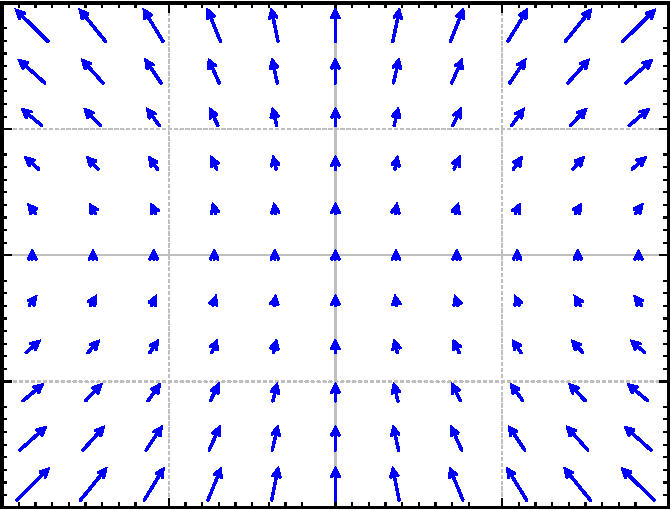
\includegraphics[width=1.75in]{figures/nlin-exer-xy-1py2}}
%\task
%\parbox[c]{1.75in}{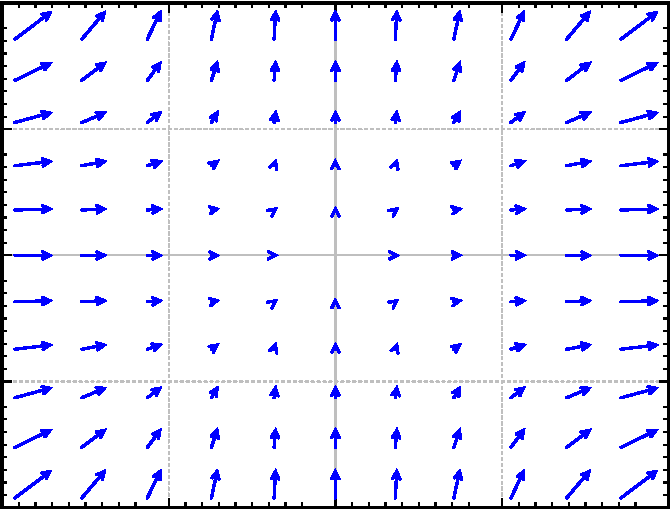
\includegraphics[width=1.75in]{figures/nlin-exer-x2-y2}}
%\task
%\parbox[c]{1.75in}{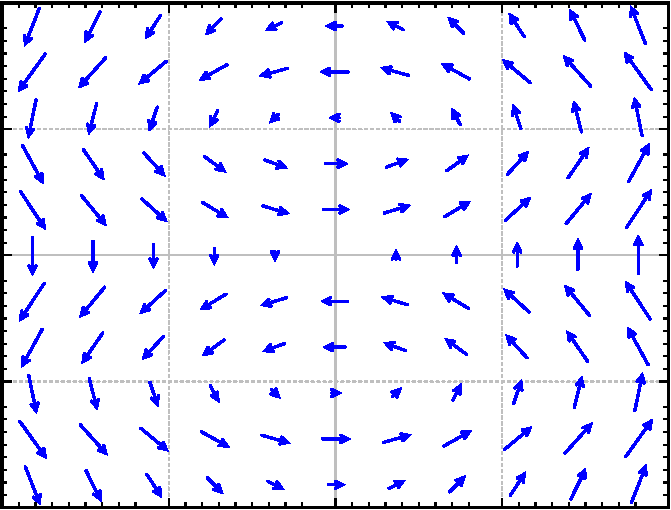
\includegraphics[width=1.75in]{figures/nlin-exer-sinpiy-x}}
%\end{tasks}
%\end{exercise}
%\end{samepage}

%\begin{exercise}\ansMark%
%Match systems
%\begin{tasks}[label=\arabic*)](2)
%\task $x'=y^2$, \enspace $y'=-x^2$,
%\task $x'=y$, \enspace $y'=(x-1)(x+1)$,
%\task $x'=y+x^2$, \enspace $y'=-x$,
%\end{tasks}
%to the vector fields below.  Justify.
%\begin{tasks}(3)
%\task \parbox[c]{1.75in}{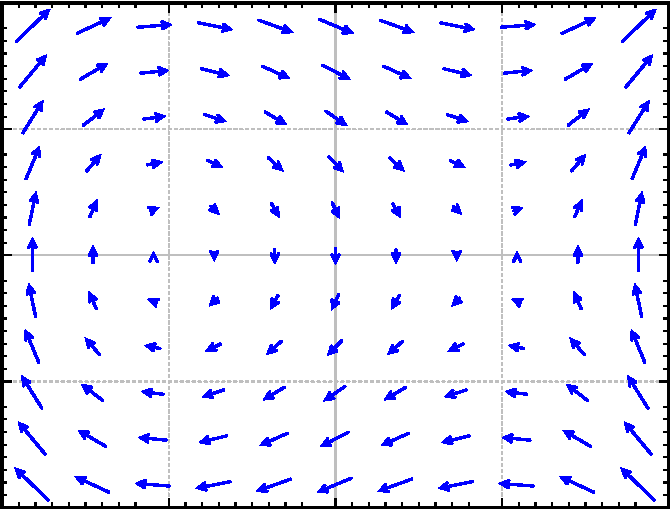
\includegraphics[width=1.75in]{figures/nlin-exer-y-xm1xp1}}
%\task \parbox[c]{1.75in}{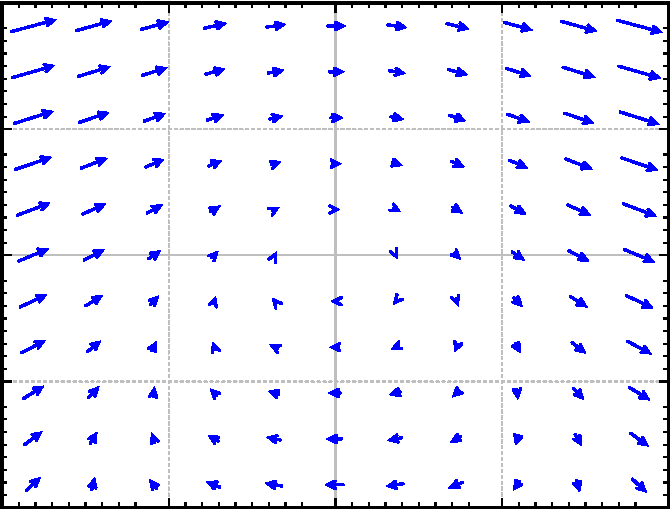
\includegraphics[width=1.75in]{figures/nlin-exer-ypx2-mx}}
%\task \parbox[c]{1.75in}{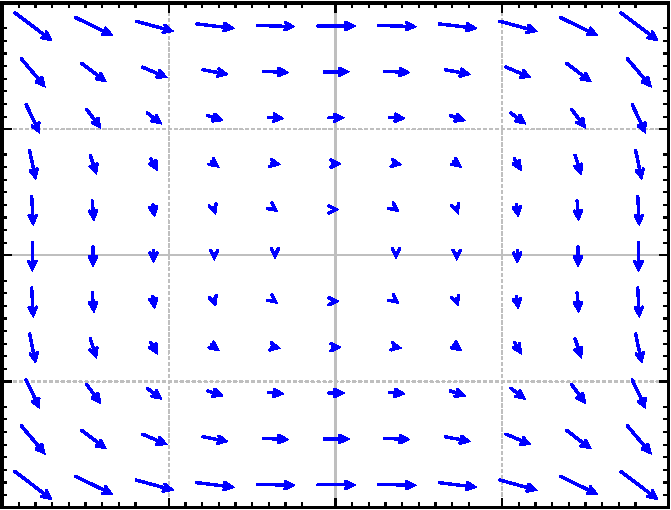
\includegraphics[width=1.75in]{figures/nlin-exer-y2-mx2}}
%\end{tasks}
%\end{exercise}
%\exsol{%
%1) is c), \quad 2) is a), \quad 3) is b)
%}


\begin{exercise}
Find the critical points and linearizations of the following systems.
\begin{tasks}(2)
\task $x'=x^2-y^2$, \enspace $y'=x^2+y^2-1$,
\task $x'=-y$, \enspace $y'=3x+yx^2$,
\task $x'=x^2+y$, \enspace $y'=y^2+x$.
\end{tasks}
\end{exercise}

\pagebreak[2]
\begin{exercise}\ansMark%
Find the critical points and linearizations of the following systems.
\begin{tasks}(2)
\task $x'=\sin(\pi y)+(x-1)^2$, \enspace $y'=y^2-y$,
\task $x'=x+y+y^2$, \enspace $y'=x$,
\task $x'=(x-1)^2+y$, \enspace $y'=x^2+y$.
\end{tasks}
\end{exercise}
\exsol{%
a) Critical points $(0,0)$ and $(0,1)$.  At $(0,0)$ using $u=x$, $v=y$ the linearization is $u'=-2u-(\nicefrac{1}{\pi})v$, $v'=-v$.
At $(0,1)$ using $u=x$, $v=y-1$ the linearization is
$u'=-2u+(\nicefrac{1}{\pi})v$, $v'=v$.\\
b) Critical point $(0,0)$.  Using $u=x$, $v=y$ the linearization is
$u'=u+v$, $v'=u$.\\
c) Critical point $(\nicefrac{1}{2},\nicefrac{-1}{4})$.  Using
$u=x-\nicefrac{1}{2}$, $v=y+\nicefrac{1}{4}$ the linearization is
$u'=-u+v$, $v'=u+v$.
}

\begin{exercise}
For the following systems, verify they have critical point at $(0,0)$,
and find the linearization at $(0,0)$.
\begin{tasks}(2)
\task $x'=x+2y+x^2-y^2$, \enspace $y'=2y-x^2$
\task $x'=-y$, \enspace $y'=x-y^3$
\task* $x'=ax+by+f(x,y)$, $y'=cx+dy+g(x,y)$, where
$f(0,0) = 0$,
$g(0,0) = 0$, and all first partial derivatives of $f$ and $g$ are
also zero at $(0,0)$, that is,
$\frac{\partial f}{\partial x}(0,0) = 
\frac{\partial f}{\partial y}(0,0) = 
\frac{\partial g}{\partial x}(0,0) = 
\frac{\partial g}{\partial y}(0,0) = 0$.
\end{tasks}
\end{exercise}

\begin{exercise}
Take the system $x' = (x-2)(x+y)$, \ $y' = (y+3)(x-y)$.
\begin{tasks}
\task Find all critical points.
\task Determine the linearization of this system around each of the critical points.
\task For each of the critical points, determine the behavior and classify the type of solution that the \emph{linearized} system will have around that critical point. 
\end{tasks}
\end{exercise}

\begin{exercise}
Take the system $x' = (x^2 - y)(x+3)$, \ $y' = (y-1)(x+y+1)$.
\begin{tasks}
\task Find all critical points.
\task Determine the linearization of this system around each of the critical points.
\task For each of the critical points, determine the behavior and classify the type of solution that the \emph{linearized} system will have around that critical point. 
\end{tasks}
\end{exercise}

\begin{exercise}
Take $x'=(x-y)^2$, \enspace $y'=(x+y)^2$. 
\begin{tasks}
\task Find the set of critical points.
\task Sketch a phase diagram and describe the behavior near the critical
point(s).
\task Find the linearization.  Is it helpful in understanding the system?
\end{tasks}
\end{exercise}

\begin{exercise}
Take $x'=x^2$, \enspace $y'=x^3$.
\begin{tasks}
\task Find the set of critical points.
\task Sketch a phase diagram and describe the behavior near the critical
point(s).
\task Find the linearization.  Is it helpful in understanding the system?
\end{tasks}
\end{exercise}

\begin{samepage}
\begin{exercise}\ansMark%
The idea of critical points and linearization works in higher dimensions as
well.  You simply make the Jacobian matrix bigger by adding more functions
and more variables.  For the following system
of 3 equations find the critical points and their linearizations:
\begin{equation*}
x' = x + z^2, \qquad y' = z^2-y, \qquad z' = z+x^2.
\end{equation*}
\end{exercise}
\end{samepage}
\exsol{%
Critical points are $(0,0,0)$, and
$(-1, 1, -1)$.
The linearization at the origin using variables $u=x$, $v=y$, $w=z$ is
$u' = u$, $v'=-v$, $z' = w$.
The linearization at the point $(-1,1,-1)$ using variables $u=x+1$,
$v=y-1$, $w=z+1$ is
%$x=u-1$
%$y=v+1$
%$z=w-1$
%$u' = u-1 + (w-1)^2$, $v' = (w-1)^2-v+1$, $w' = (w-1)+(u-1)^2$.
%$u' = u + w^2-2w$, $v' = w^2-2w-v$, $w' = w+u^2-2u$
$u'=u-2w$, $v'=-v-2w$, $w'=w-2u$.
}

\begin{exercise}\ansMark%
Any two-dimensional non-autonomous system $x'=f(x,y,t)$, $y'=g(x,y,t)$ can
be written as a three-dimensional autonomous system (three equations).  Write down this
autonomous system using the variables $u$, $v$, $w$.
\end{exercise}
\exsol{%
$u' = f(u,v,w)$, $v'=g(u,v,w)$, $w' = 1$.
}

\setcounter{exercise}{100}

